\documentclass[10pt]{article}
\usepackage[letterpaper,margin=0.78in]{geometry}
\usepackage{amsmath,amssymb,bm}
\usepackage{booktabs,tabularx,array}
\usepackage{graphicx,float}
\usepackage{xcolor}
\usepackage{microtype}
\usepackage[hidelinks]{hyperref}
\usepackage[font=small,labelfont=bf]{caption}
\newcolumntype{Y}{>{\raggedright\arraybackslash}X}
\newcommand{\C}{\mathbb C}
\newcommand{\R}{\mathbb R}
\newcommand{\tr}{\operatorname{tr}}
\title{\vspace{-1.4em}\textbf{Fixed-Geometry In-Context Linear Sampling\\with Learned Acquisition Design}\\[-0.15em]
\large A two-dimensional proof of concept}
\author{}
\date{August 4, 2026}

\begin{document}
\maketitle
\vspace{-2.0em}

\begin{abstract}
We test a fixed-feature in-context architecture on the actual linear sampling
method (LSM), rather than on one-dimensional Gaussian-process regression.  Each
task is a two-dimensional active multistatic inverse-scattering problem with a
complex far-field matrix.  A prescribed angular softmax kernel defines the GP
feature geometry.  A tied complex preconditioned conjugate-gradient (PCG) loop
then solves all Bayesian LSM sampling equations in context.  Only a positive
preconditioner built from the fixed attention geometry is trained; no
temperature, image surrogate, indicator, noise estimator, or spatial
regularization map is learned.  Across three independent seeds and 576 held-out
tasks per condition, the 20-loop model matches direct Tikhonov localization at
15\% relative noise, including unseen kites and two-obstacle configurations,
while attaining mean relative sampling-equation residuals between $1.0\times
10^{-2}$ and $1.8\times10^{-2}$.  A controlled recurrent-solver ablation shows
that heavy-ball and Chebyshev iterations can localize at the same depth, but
leave residuals above $0.54$; Richardson requires about 80 loops even for
localization.  In a second proof of concept, six continuous
source/receiver angles are trained end to end.  The learned design reaches
average precision $0.958/0.963/0.879$ on ellipses/kites/two obstacles, versus
$0.260/0.263/0.244$ for six uniformly spaced angles.  A point-spread audit
attributes this gain to suppression of periodic grating lobes.  These results
support the mechanism and experiment-design idea, but remain a synthetic
Born--Foldy study rather than a full sound-soft validation.
\end{abstract}

\section{Question tested and precise scope}

The experiment asks whether a prescribed nonlinear kernel geometry can be
combined with a tied in-context loop to solve LSM systems, and whether the same
differentiable pipeline can optimize an acquisition geometry.  It does
\emph{not} learn a map from a response matrix to an obstacle image.

The physical regime is two-dimensional, active, deterministic and multistatic.
There are 32 fixed plane-wave incident directions and 32 fixed receiver
directions on a full circle.  The randomness across tasks lies in the obstacle
and measurement noise, not in the sources.  Consequently this first proof of
concept uses the far-field matrix $F_D$ and is distinct from the random-source
cross-correlation matrix $C_D$ in Garnier--Haddar--Montanelli~\cite{ghm2023} and
the mean-removed matrix $\widetilde C_D$ generated by a moving small random
scatterer~\cite{ghm2024}.

It is also distinct from Chenu--Haddar--Montanelli~\cite{chm2026}.  Their neural
operator learns an indicator-dependent regularization function before a
classical LSM solve.  Here the indicator is never represented by a neural
network: the recurrent cell itself executes the sampling solve, and the
nonlinear feature kernel is fixed by construction.

\section{Two-dimensional LSM task}

Let $\widehat x_r,d_s\in\mathbb S^1$ be receiver and incident directions and
let $D_h$ be the grid representation of an obstacle.  The fast training-only
forward model is the Born--Foldy sum
\begin{equation}
 (F_D)_{rs}
 =\frac{1}{|D_h|}\sum_{y\in D_h}
 \exp\!\left\{ik(d_s-\widehat x_r)\cdot y\right\}+E_{rs},
 \qquad F_D\in\C^{m\times m}.
 \label{eq:born}
\end{equation}
For every probing point $z\in\Omega\subset\R^2$, the LSM right-hand side is
\begin{equation}
 (\phi_z)_r=\exp(-ik\widehat x_r\cdot z).
\end{equation}
Training shapes are disks and ellipses.  Kites and pairs of disks are held out
as geometric out-of-distribution (OOD) tests.  The main configuration uses
$m=32$, $k=8$, a $32\times32$ probing grid on $[-0.8,0.8]^2$, and relative
complex Gaussian noise drawn between 3\% and 12\% during training.  Evaluation
uses 8\% and 15\% noise.

\section{Fixed nonlinear GP geometry}

For acquisition angles $\theta_j$, the prescribed von Mises kernel and its
row-normalized nonlinear attention are
\begin{equation}
 W_{j\ell}=\exp\{\gamma\cos(\theta_j-\theta_\ell)\},
 \qquad S_{j\ell}=\frac{W_{j\ell}}{\sum_p W_{jp}}.
 \label{eq:softmax}
\end{equation}
The positive GP covariance is
\begin{equation}
 K_g=(1-\rho)I+\rho D_W^{-1/2}WD_W^{-1/2},
 \qquad \gamma=1,\quad \rho=0.2.
 \label{eq:prior}
\end{equation}
Both $\gamma$ and $\rho$ are modelling choices.  They are buffers, not learned
parameters or temperatures.  With residual scale $\lambda_D$, Bayesian least
squares gives the dual system
\begin{equation}
 H_Dq_z=\phi_z,\qquad
 H_D=F_DK_gF_D^*+\lambda_DI,\qquad
 g_z=K_gF_D^*q_z,
 \label{eq:dual}
\end{equation}
and the reported LSM score is
\begin{equation}
 s_D(z)=-\frac12\log\!\left(g_z^*K_g^{-1}g_z\right).
 \label{eq:indicator}
\end{equation}

\section{Tied in-context architecture}

Jacobi scaling and a row-sum bound are applied to~\eqref{eq:dual}, without an
eigendecomposition.  Denote the scaled Hermitian positive operator by $A_D$
and its right-hand side by $b_z$.  The recurrent cell is complex PCG.  With
$r_0=b_z$, $u_0=0$ and $p_0=P_Dr_0$, it applies
\begin{align}
 \alpha_t&=\frac{\langle r_t,P_Dr_t\rangle}
 {\langle p_t,A_Dp_t\rangle},
 &u_{t+1}&=u_t+\alpha_tp_t,\\
 r_{t+1}&=r_t-\alpha_tA_Dp_t,
 &\beta_t&=\frac{\langle r_{t+1},P_Dr_{t+1}\rangle}
 {\langle r_t,P_Dr_t\rangle},\\
 p_{t+1}&=P_Dr_{t+1}+\beta_tp_t.&&
 \label{eq:pcg}
\end{align}
The same cell and preconditioner are reused at every depth.  To incorporate the
fixed nonlinear attention without corrupting Krylov conjugacy, the learned
object is constrained to be SPD:
\begin{equation}
 L_\Gamma=I-D_W^{-1/2}WD_W^{-1/2},\qquad
 P_D=I+a_DL_\Gamma+b_DL_\Gamma^2,\qquad a_D,b_D\ge0.
 \label{eq:preconditioner}
\end{equation}
A small invariant controller reads six scalar summaries of $A_D$ once and
returns $(a_D,b_D)$.  It does not see spatial query coordinates and cannot emit
an image.  The exact CG coefficients in~\eqref{eq:pcg} are computed from the
prompt $(F_D,\phi_z)$, which is the in-context computation.

The training loss is a balanced pairwise ranking loss between interior and
exterior probing points plus $0.2\log(1+\|r_T\|/\|b\|)$.  A direct solve is
never used as a training target.  Direct Tikhonov appears only as a held-out
reference.  Each of three seeds uses 1500 gradient steps, batch size 16 and
AdamW at learning rate $10^{-3}$.

\section{Fixed-geometry results}

Table~\ref{tab:fixed} reports 15\% noise.  Each entry pools 576 independent
tasks (192 per seed); uncertainty is a 95\% confidence interval over tasks.
The eight-loop indicator is already accurate although its algebraic residual
is not yet small.  At 20 loops, learned PCG and the direct solve are visually
and statistically indistinguishable.  The learned SPD preconditioner reduces
the OOD-kite mean residual from $0.830$ to $0.746$ at eight loops and from
$0.0141$ to $0.0102$ at 20 loops.

\begin{table}[H]
\centering
\caption{Average precision at 15\% noise; mean $\pm$ 95\% CI.}
\label{tab:fixed}
\begin{tabular}{lccc}
\toprule
Method & ellipse (ID) & kite (OOD) & two disks (OOD)\\
\midrule
identity CG, 8 loops & $0.9915\pm0.0006$ & $0.9879\pm0.0008$ & $0.9135\pm0.0028$\\
trained PCG, 8 loops & $0.9915\pm0.0007$ & $0.9881\pm0.0008$ & $0.9136\pm0.0028$\\
trained PCG, 20 loops & $0.9917\pm0.0006$ & $0.9889\pm0.0008$ & $0.9131\pm0.0028$\\
direct Tikhonov & $0.9917\pm0.0006$ & $0.9889\pm0.0008$ & $0.9131\pm0.0028$\\
\bottomrule
\end{tabular}
\end{table}

\begin{figure}[H]
\centering

\includegraphics[width=\linewidth]{fixed_geometry_reconstructions.png}
\caption{Three unseen kites at 8\% noise.  The output is the LSM score obtained
from recurrently computed $g_z$, not a neural image prediction.}
\label{fig:fixed-reconstruction}
\end{figure}

The depth audit separates image quality from solver fidelity.  Average
precision saturates after roughly four loops, whereas the residual continues
to fall by two orders of magnitude through depth 20.  On an H100, a batch of
24 matrices and all 1024 probing points takes 11.69\,ms at eight loops,
15.53\,ms at 20 loops, and 15.51\,ms for the direct solve.  Thus this small
$32\times32$ experiment establishes computational structure, not a large-scale
speed advantage.

\begin{figure}[H]
\centering
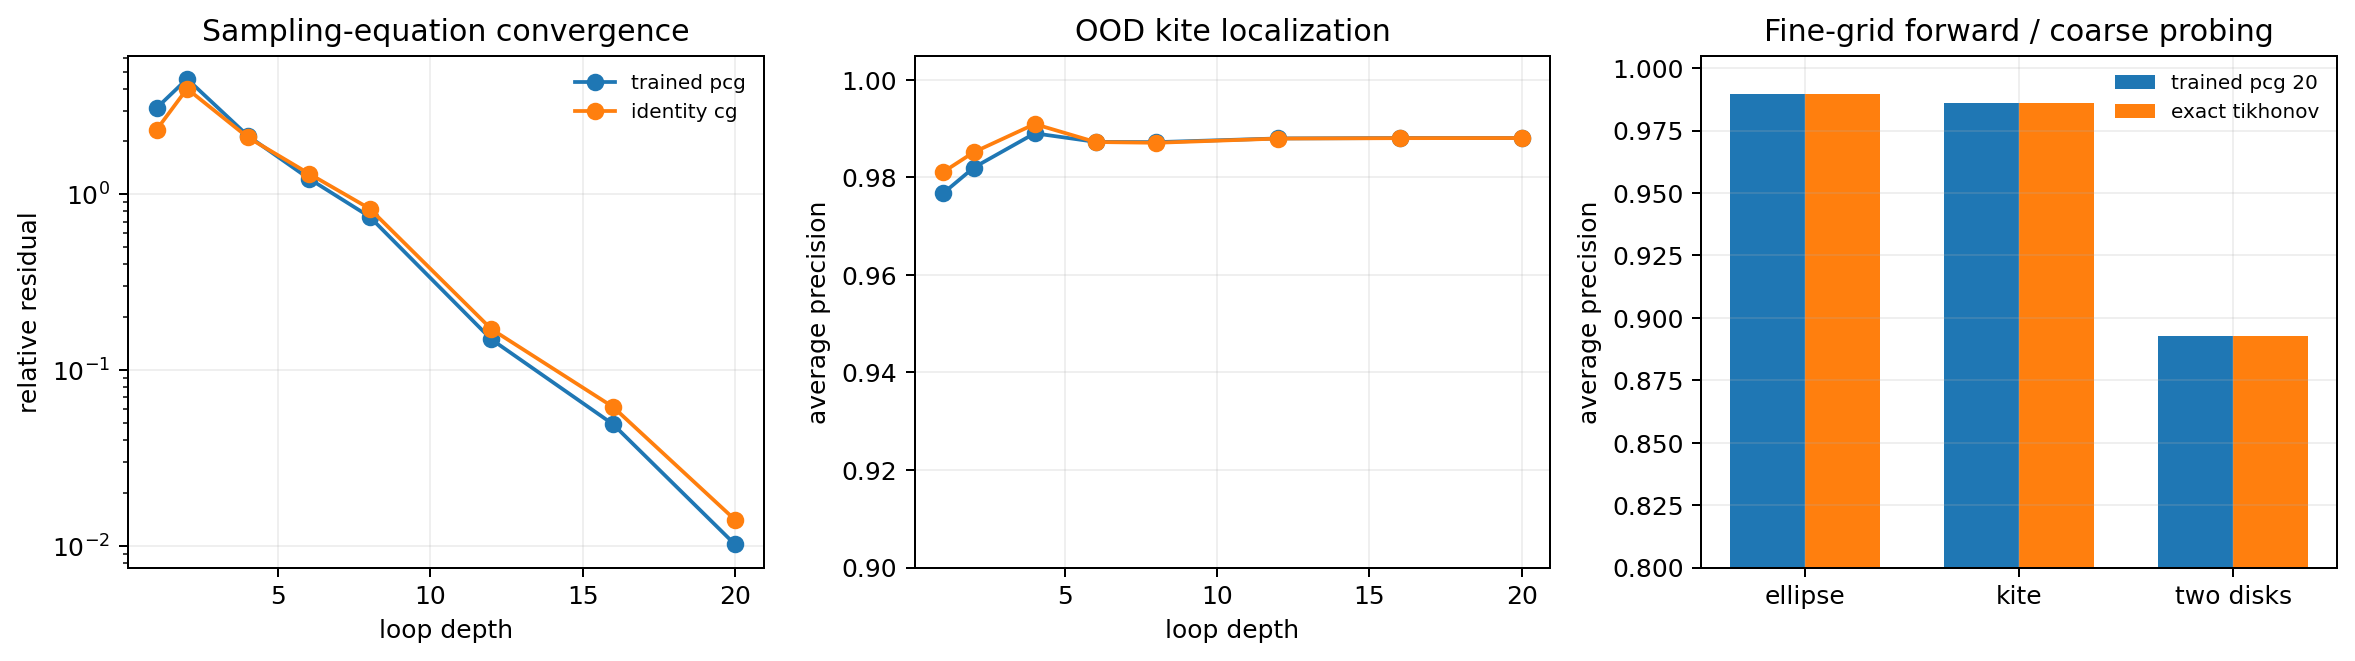
\includegraphics[width=\linewidth]{depth_and_offgrid.png}
\caption{Left: convergence of the sampling equation.  Middle: localization
saturates before the algebraic solve.  Right: the fine-grid forward control
uses a $64^2$ scattering grid and a separate $32^2$ probing grid.}
\label{fig:depth-offgrid}
\end{figure}

The separate-grid control rules out the simplest inverse crime.  With data
assembled on $64^2$ points but probing on $32^2$, trained PCG retains average
precision $0.9896/0.9858/0.8926$ on ellipses/kites/two disks, exactly matching
the direct-solve ranking to four decimals.

\section{Controlled recurrent-solver ablation}

This is a small ICL experiment.  The controller is a
$6\!\to\!32\!\to\!32\!\to\!2$ MLP with 1,346 trainable parameters (5.3,kB in
single precision).  To isolate the effect of the iterative method, Richardson,
heavy-ball, Chebyshev and PCG use exactly the same six invariant summaries of
$A_D$, the same fixed GP kernel, the same Bayesian system~\eqref{eq:dual}, the
same score decoder~\eqref{eq:indicator}, training tasks, loss, depth, seeds and
optimizer.  Only the recurrent update changes.  In particular, the stationary
baselines take the form
\begin{align}
 u_{t+1}^{\mathrm R}
 &=u_t+\eta_D(b-A_Du_t),\label{eq:richardson}\\
 u_{t+1}^{\mathrm{HB}}
 &=u_t+\eta_D(b-A_Du_t)+\beta_D(u_t-u_{t-1}),\label{eq:hb}
\end{align}
where the controller selects stable task-conditioned coefficients.  The
Chebyshev semi-iteration uses the same second-order recurrence, with its
coefficients generated from controller-selected spectral bounds
$[\ell_D,L_D]$.  Thus it learns an iteration polynomial, not a reconstruction
map.  PCG instead preserves exact in-context Krylov coefficients and uses the
controller output only in the SPD preconditioner~\eqref{eq:preconditioner}.

Table~\ref{tab:solver-ablation} exposes an important distinction.  At 20 loops,
heavy-ball and Chebyshev already produce good indicator rankings, but they have
not solved the sampling equations: their OOD-kite residuals are $0.591$ and
$0.544$, compared with $0.010$ for PCG.  Richardson fails both tests at this
depth.  The conclusion is therefore not that all loops are interchangeable;
localization is insensitive to sizeable coefficient error, whereas Bayesian
least-squares fidelity is not.

\begin{table}[H]
\centering
\small
\caption{Same-encoder/same-decoder comparison at 20 loops and 15\% noise.
Average precision (AP) and kite residual pool 576 tasks; runtime is milliseconds
for a batch of 24 matrices and all 1024 probing points on an H100.}
\label{tab:solver-ablation}
\begin{tabular}{lrrrrr}
\toprule
Loop & parameters & ellipse AP & kite AP & two-disks AP & kite residual \\
\midrule
Richardson & 1,346 & 0.1062 & 0.1187 & 0.0470 & 0.7699 \\
heavy-ball & 1,346 & 0.9856 & 0.9838 & 0.8690 & 0.5911 \\
Chebyshev & 1,346 & 0.9802 & 0.9886 & 0.8691 & 0.5438 \\
PCG & 1,346 & 0.9926 & 0.9890 & 0.9118 & 0.0101 \\
direct Tikhonov & 0 & 0.9926 & 0.9890 & 0.9118 & $1.7\times10^{-5}$ \\
\bottomrule
\end{tabular}
\end{table}

The cost per 20-loop batch is 11.45,ms for Richardson, 10.99,ms for
heavy-ball, 11.39,ms for Chebyshev and 15.01,ms for PCG.  The modest PCG
overhead buys much faster algebraic convergence.  On held-out kites,
Chebyshev reaches residual $0.214$ at 48 loops and $0.064$ at 80 loops;
heavy-ball reaches $0.265$ and $0.122$.  PCG reaches $9.6\times10^{-3}$ at 20
loops and $3\times10^{-4}$ at 32 loops.  Richardson only reaches AP $0.956$ at
80 loops, while its residual remains $0.644$.

\begin{figure}[H]
\centering
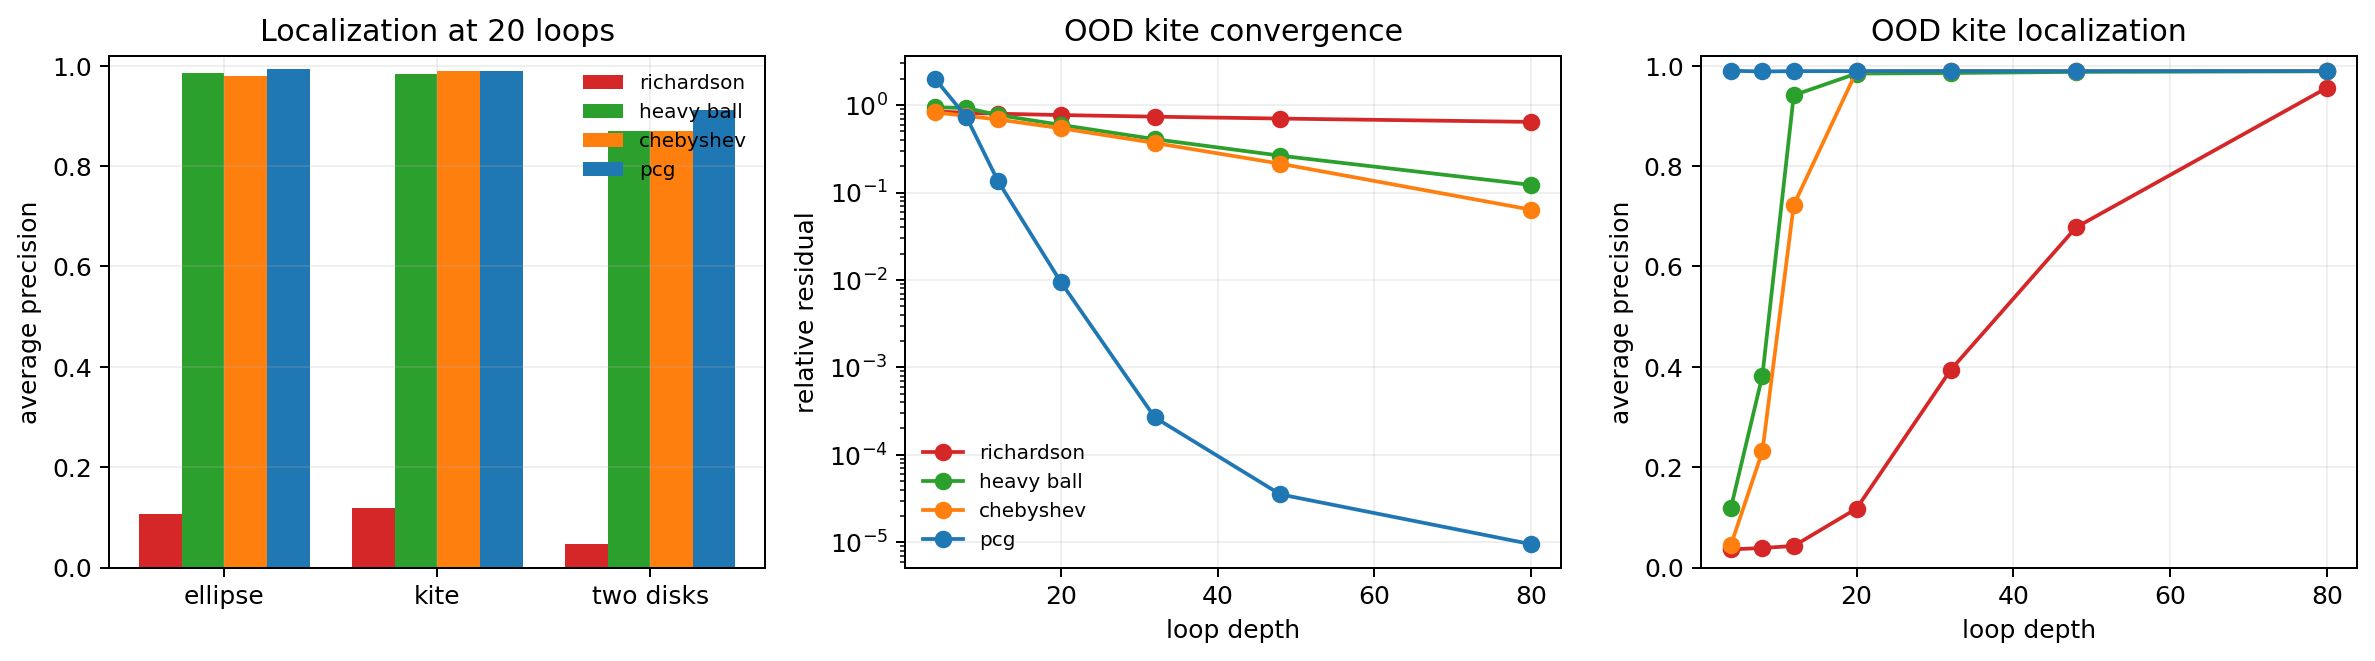
\includegraphics[width=\linewidth]{../results_solver_comparison_20260804/solver_comparison.png}
\caption{Controlled loop comparison.  Left: localization at the training
depth.  Middle: algebraic convergence on unseen kites.  Right: localization
can saturate long before the sampling system is solved.}
\label{fig:solver-comparison}
\end{figure}

\begin{figure}[H]
\centering
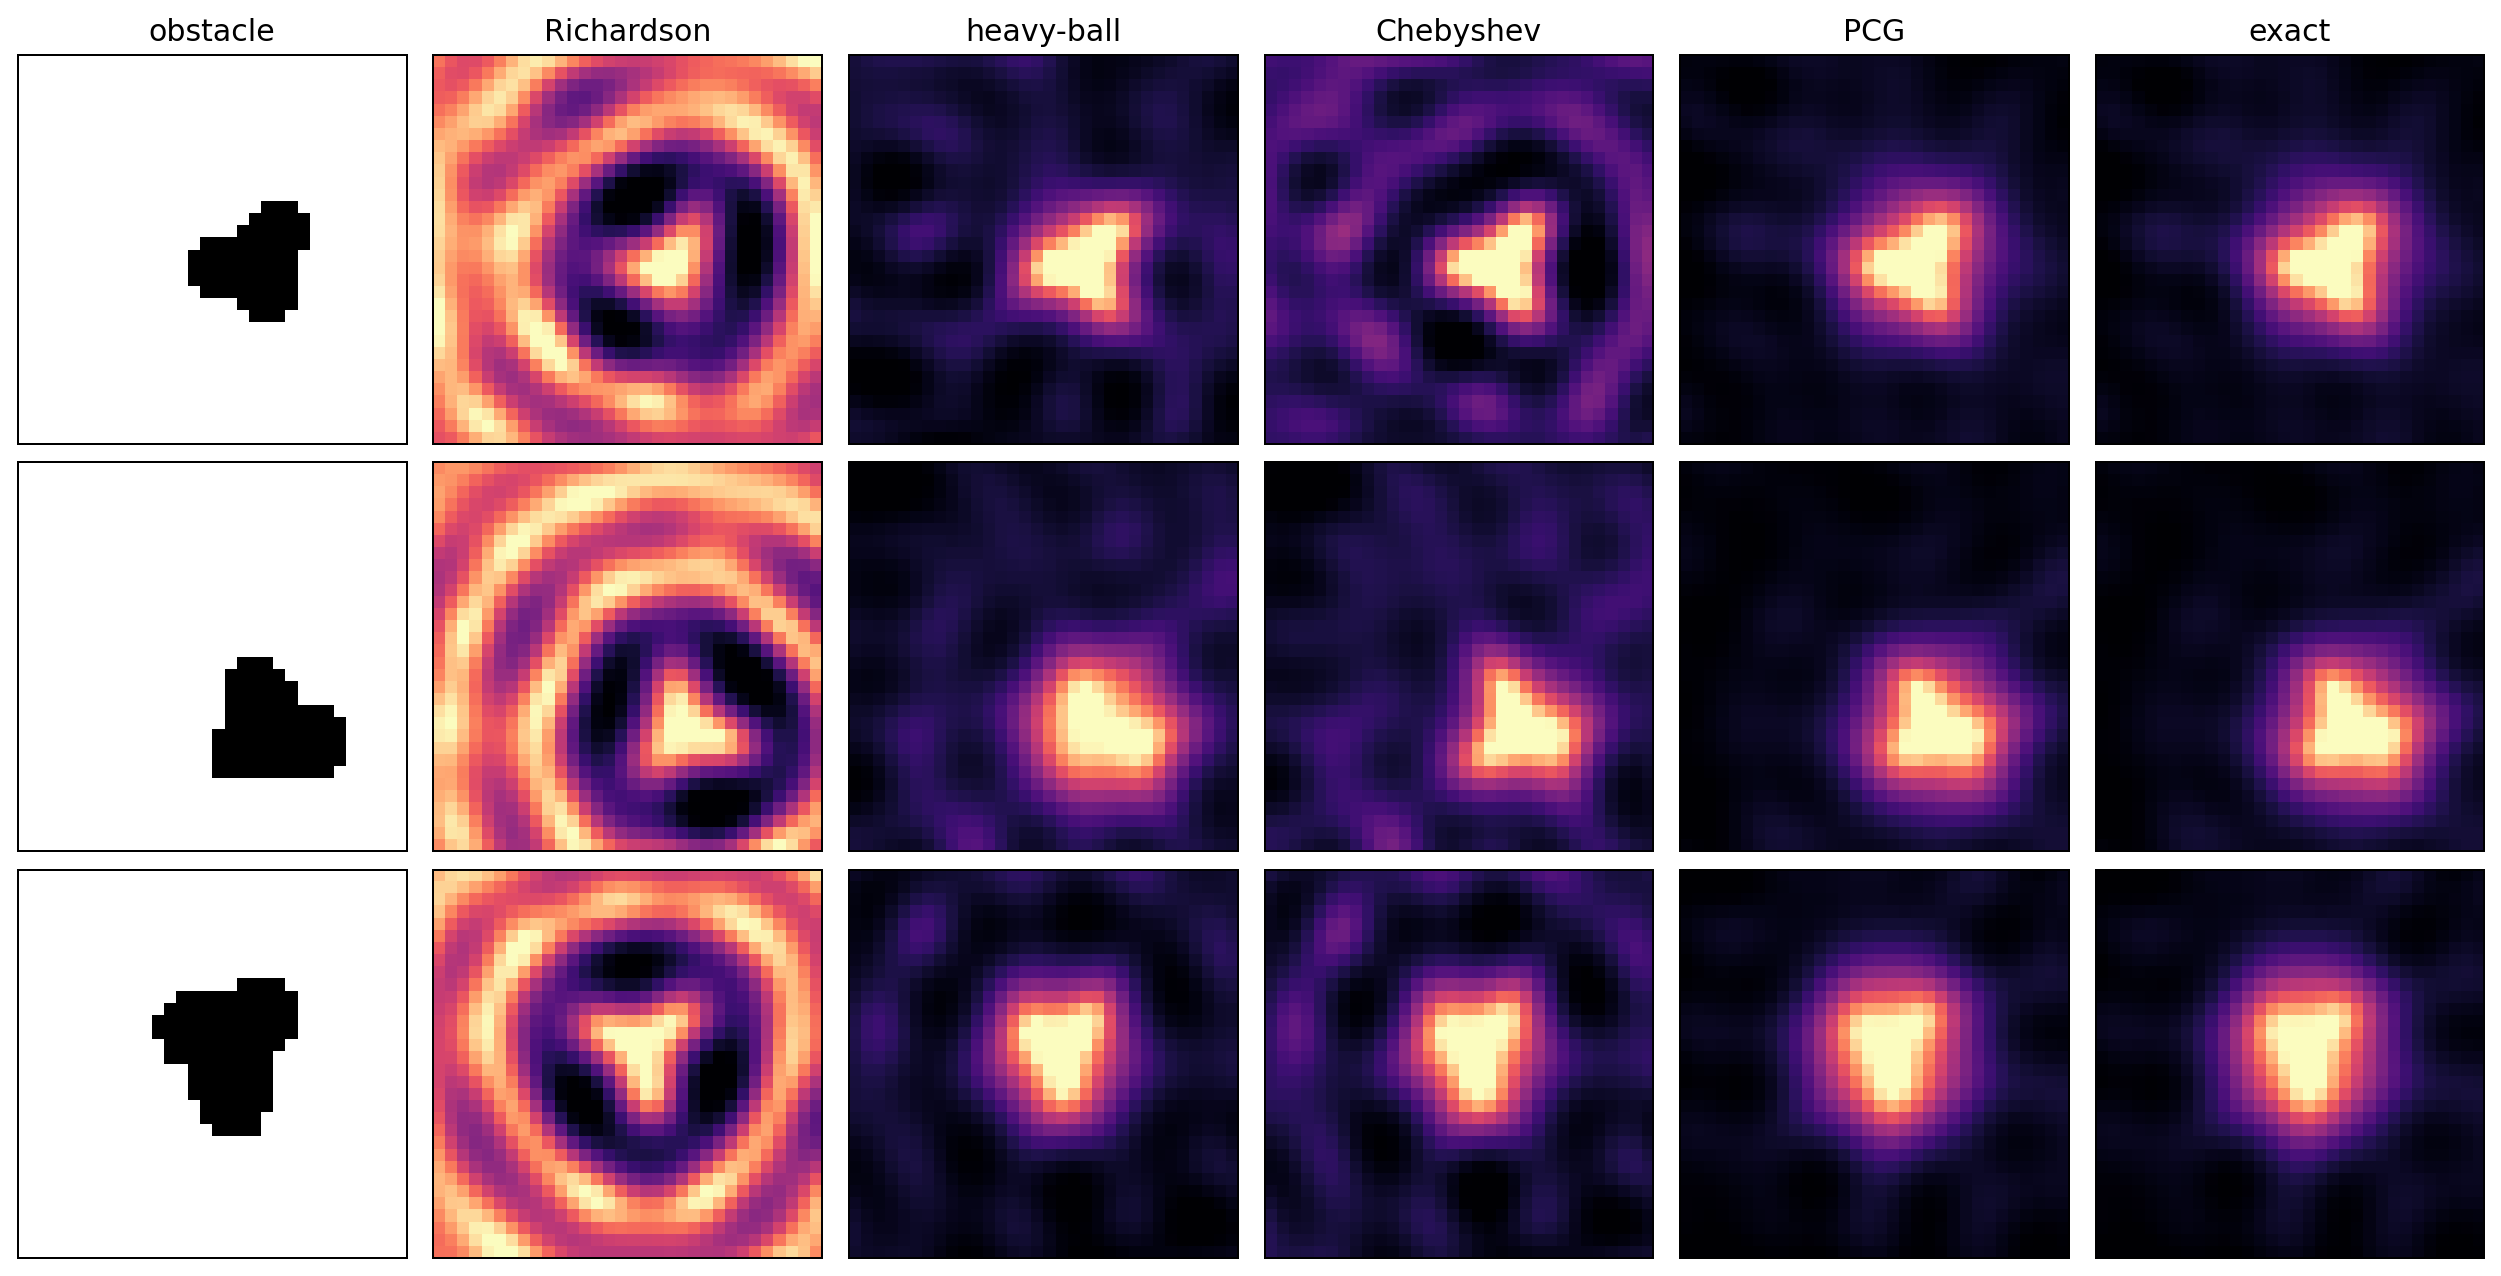
\includegraphics[width=\linewidth]{../results_solver_comparison_20260804/reconstructions.png}
\caption{Representative unseen kites at 15\% noise after 20 loops.  Heavy-ball
and Chebyshev localize the obstacle but retain structured artefacts; PCG is
visually indistinguishable from the direct Bayesian LSM solve.}
\label{fig:solver-reconstructions}
\end{figure}

\section{Learned experiment design}

The second experiment trains six shared source/receiver angles through the
frozen LSM loop.  A periodic gap parameterization enforces at least $28^\circ$
between distinct angles; hence repeated measurements cannot masquerade as new
directions.  The only optimized objective is the same LSM ranking loss.  The
baseline designs are six equally spaced angles and the random feasible
initialization for each seed.

\begin{table}[H]
\centering
\caption{Six-angle design at 12\% noise; average precision, mean $\pm$ 95\% CI.}
\label{tab:design}
\begin{tabular}{lccc}
\toprule
Design & ellipse (ID) & kite (OOD) & two disks (OOD)\\
\midrule
learned & $0.9582\pm0.0037$ & $0.9628\pm0.0034$ & $0.8790\pm0.0055$\\
random feasible & $0.8972\pm0.0083$ & $0.9090\pm0.0071$ & $0.8136\pm0.0088$\\
uniform & $0.2604\pm0.0018$ & $0.2626\pm0.0018$ & $0.2439\pm0.0019$\\
\bottomrule
\end{tabular}
\end{table}

\begin{figure}[H]
\centering

\includegraphics[width=\linewidth]{experiment_design.png}
\caption{A representative learned geometry and aggregate performance over
three design seeds.  Independent seeds converge to rotations of a similar
nonuniform paired-angle pattern.}
\label{fig:design}
\end{figure}

The poor uniform baseline is not a solver failure: its six-dimensional PCG
residual is below $10^{-4}$.  It is an acquisition ambiguity.  For the
discrete multistatic wave-vector set $k(d_s-\widehat x_r)$, uniform spacing
creates periodic replicas.  The maximum point-spread sidelobe is
$0.999\pm0.000$ for the uniform design, $0.678\pm0.104$ for the random design,
and $0.562\pm0.008$ for the learned design.

\begin{figure}[H]
\centering
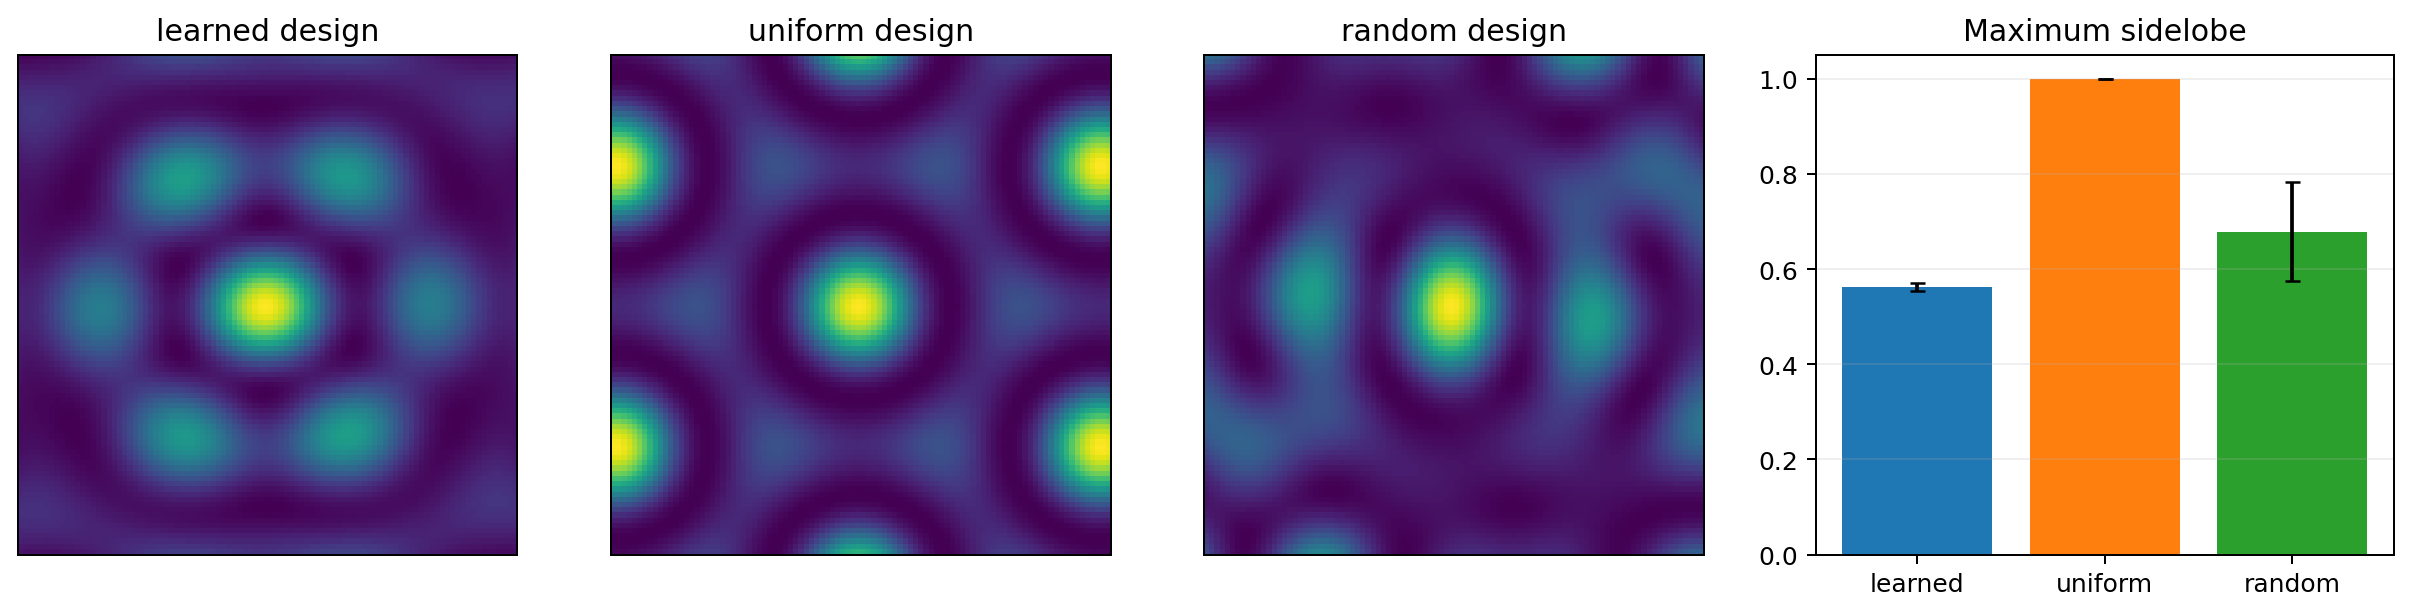
\includegraphics[width=\linewidth]{point_spread_diagnostics.png}
\caption{Central point-spread functions for one seed and maximum sidelobe over
three seeds.  The learned design suppresses the grating-lobe replicas of the
uniform six-angle array.}
\label{fig:psf}
\end{figure}

\section{What worked, what did not, and the bottleneck}

Three conclusions are supported by the data.
\begin{enumerate}
\item A fixed nonlinear acquisition kernel can be embedded in a tied complex
LSM loop without learning the feature geometry or an image surrogate.
\item Good-looking indicators do not imply a faithful sampling solve.
Heavy-ball and Chebyshev preserve useful low-frequency localization modes at
20 loops but leave residuals two orders of magnitude above PCG.  Learning
arbitrary damping factors inside CG is still less safe because it also breaks
Krylov conjugacy; constraining learning to the SPD preconditioner in
\eqref{eq:preconditioner} avoids that failure.
\item At this scale, the dominant gain comes from acquisition design, not from
the learned preconditioner.  The preconditioner improves residual convergence
modestly; choosing non-aliased angles changes reconstruction quality
dramatically.
\end{enumerate}

The principal bottleneck is therefore no longer the reconstruction map.  LSM
localizes the obstacle after few Krylov steps, while faithful posterior
coefficients require more depth.  For a presentation, image metrics must be
shown together with the sampling-equation residual; otherwise an attractive
indicator can conceal an invalid solve.

\section{Limitations and next experiment}

This is a proof of mechanism, not a publishable physical benchmark.  The
forward map~\eqref{eq:born} is a Born--Foldy discretization, not a boundary
integral solver for extended sound-soft obstacles.  All data are synthetic,
the wavenumber and circular aperture are fixed, and obstacle masks supervise
the ranking loss.  The fine-grid control removes exact grid reuse but not model
mismatch.  Most importantly, no claim is made yet for passive random-source
LSM or for the small-random-scatterer construction.  Those settings require
training on $C_D$ or $\widetilde C_D$ while varying the number of sources,
realizations, receivers and aperture.  Scaling laws should be fitted only
after those physically distinct experiments exist.

The next decisive test is to replace~\eqref{eq:born} by an independent
sound-soft boundary-integral simulator, retain the frozen kernel and PCG cell,
and evaluate the already trained loop without fine-tuning.  Only then should
the random-source regimes be added.

\section*{Reproducibility}

All tasks are generated online.  Seeds are 17, 29 and 43.  The primary run took
164 seconds and the controlled four-solver audit took 216 seconds on one NVIDIA
H100 PCIe, excluding document compilation.  The release contains task-level
CSV files, confidence summaries, checkpoints, figures, protocol metadata,
tests and the exact commands in the README.

\begin{thebibliography}{9}
\bibitem{ghm2023}
J.~Garnier, H.~Haddar, and H.~Montanelli.
\newblock The linear sampling method for random sources.
\newblock \emph{arXiv:2210.15560}, 2023.

\bibitem{ghm2024}
J.~Garnier, H.~Haddar, and H.~Montanelli.
\newblock The linear sampling method for data generated by small random
scatterers.
\newblock \emph{arXiv:2403.19482}, 2024.

\bibitem{chm2026}
V.~Chenu, H.~Haddar, and H.~Montanelli.
\newblock A neural operator framework for solving inverse scattering problems.
\newblock \emph{arXiv:2602.24147}, 2026.
\end{thebibliography}

\end{document}
